\documentclass[10pt]{article}
\usepackage[paper=letterpaper,margin=2cm]{geometry}
\usepackage{amsmath}
\usepackage{amssymb}
\usepackage{amsfonts}
\usepackage{newtxtext, newtxmath}
\usepackage{enumitem}
\usepackage{titling}
\usepackage{graphicx}    %  in the preamble
\usepackage{fancyhdr}
\usepackage[colorlinks=true]{hyperref}

\setlength{\droptitle}{-10em}

\fancyhf{}
\fancyhead[L]{MATH 232: Linear Algebra}
\fancyhead[R]{Steven Wong, 301337727}
\renewcommand\headrulewidth{0pt}
\pagestyle{fancy}

\begin{document}

\noindent\makebox[\textwidth][c]{\Large\bfseries Assignment 2}
\normalsize
\begin{enumerate}[leftmargin=\labelsep]
    \item[1A.)] Let $x_1 = (2, 5) \text{and let } x_2 = (8, 13)$. Working with vectors $x_1$ and $x_2$, I have elected to apply a stretch in the x-direction by a factor of a 5, and a reflection across the y-axis. These are denoted by the following matrix operators: 
    
    $$
    \textbf{X-Direction Stretch: }\begin{bmatrix} 5 & 0 \\ 0 & 1
    \end{bmatrix},\:
    \textbf{Y-Axis Reflection: }\begin{bmatrix} -1 & 0 \\ 0 & 1
    \end{bmatrix}
    $$
    
    We obtain the following results by multiplying vectors $x_1$ and $x_2$ by these transformation matrices and plotting their resulting rectangles where black is our original plot, red is our x-direction stretch, and blue as our reflection across the y-axis. \textbf{LOOK INTO WAYS TO ANNOTATE FIGURES}
    
    \begin{center}
        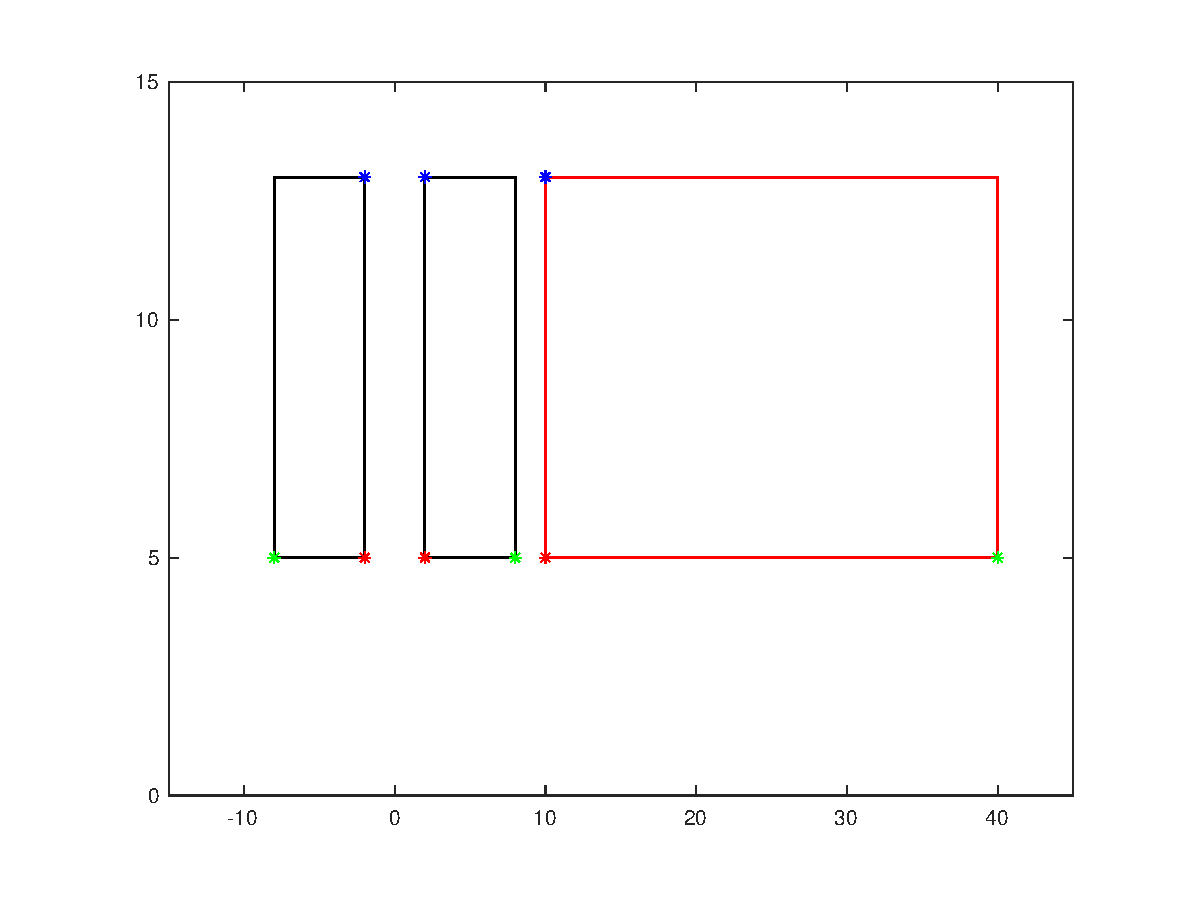
\includegraphics[scale=0.5]{Figure1.eps}
    \end{center}
    
    \item[1B.)] For Part1B Composition: Verify the result of Problem A6 in Section 3.3 of the text; that the two compositions of a vertical shear and a stretch in the y direction, do not commute. Do this by plotting the image of the unit square with corners at (1, 1),(2, 1),(2, 2),(1, 2). Then plot the results of applying the COMPOSITION of the two operations (vertical shear and stretch) in both orders and showing that the resulting shape depends on the order in which the operations are applied. Corroborate your ’experimental proof’ of the non-commutability of these transformations by referring to Theorem 3.2.5 of the text (i.e., by considering the associated matrices).
    
    \item[2.A)] Manipulating an image: Find the matrix that transforms the black rectangle into the red rectangle. Look at the diagram and observe what has happened to the black rectangle. Form the matrices that do these operations; there are two. Multiply these matrices in the correct order to get the transformation matrix A. Experimentally verify that you can plot the black rectangle yourself and then multiply the vectors that describe the opposite vertices by A and obtain and plot the red rectangle. Include the matrices you used to do this in your report.
    
    The first matrix reflects the black rectangle over the y-axis 
    
     $$
    \textbf{First matrix operation: }\begin{bmatrix} -1 & 0 \\ 0 & 1
    \end{bmatrix}
    $$
    

\end{enumerate}
\end{document}


    $$
    \textbf{X-Direction Stretch: }\begin{bmatrix} 5 & 0 \\ 0 & 1
    \end{bmatrix},\:
    \textbf{Y-Axis Reflection: }\begin{bmatrix} -1 & 0 \\ 0 & 1
    \end{bmatrix}
    $$